\section{Results}
\label{sec:results}

In this section, we provide relevant details pertaining to the construction of the surrogate model to predict
the field of interest, i.e. the
residual stress in the AM part cross-section using the PCAS method in~\ref{sub:surr}. The surrogate is used to map
the process control parameters and the material properties to the residual stress field. The computational efficiency
enabled by the surrogate is exploited to perform a global sensitivity analysis of the inputs in~\ref{sub:gsa}. Finally, the
surrogate is used for reliability prediction for the AM part by estimating the probability of failure based on residual stress
in~\ref{sub:reliability}.

\subsection{Surrogate Model}
\label{sub:surr}

A surrogate model is constructed for the residual stress field at the cross-section of the part 
(x-z plane in Figure~\ref{fig:PartwMesh}) passing through its center. We will refer to this plane
as x$^c$-z$^c$ in the remainder of this paper. The surrogate maps three sets of
parameters, namely, the process control parameters~($\bm{\theta_P}$), mechanical properties~($\bm{\theta_M}$),
and thermal properties~($\bm{\theta_T}$) to the stress field. The set of process control parameters includes
the beam power~($P$), scan speed~($v$), and the pre-heat temperature~($T_0$). Mechanical properties
include the yield strength~($Y$), the elastic modulus~($E$), and the bulk density~($\rho$). Thermal 
properties include specific heat~($C_p$) and bulk thermal conductivity~($\kappa$). Note that $C_p$ and $\kappa$
are considered to be functions of the local temperature, $T$. Specifically, a polynomial of degree 2 was fit
to a set of data pertaining to the variation of $C_p$ and $\kappa$ with temperature (20~K--1655~K), 
provided in~\cite{Fu:2014} as shown in Figure~\ref{fig:Cp_kappa}.
%
\begin{figure}[htbp]
\begin{center}
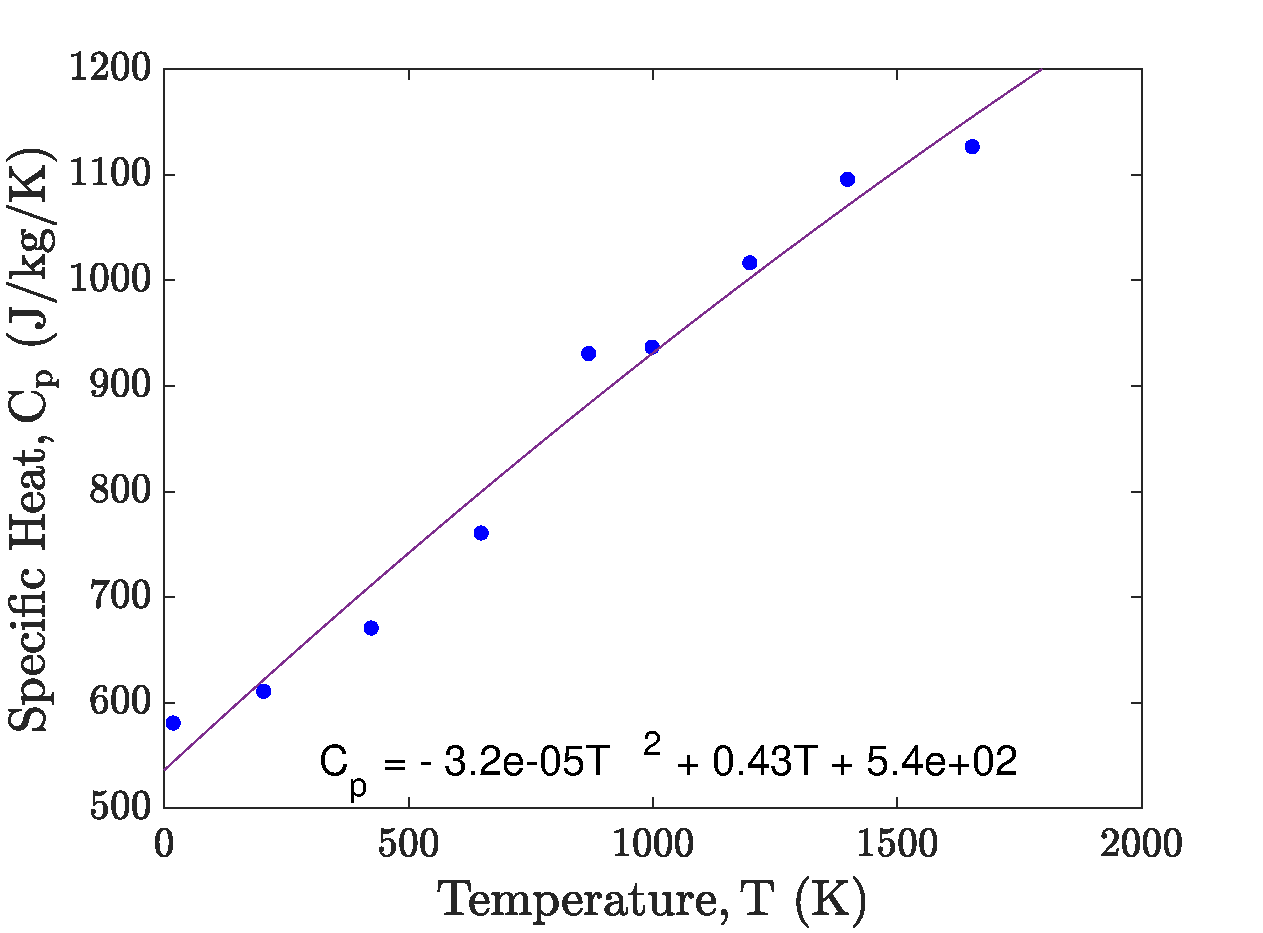
\includegraphics[width=0.42\textwidth]{./Figures/cp_fit}
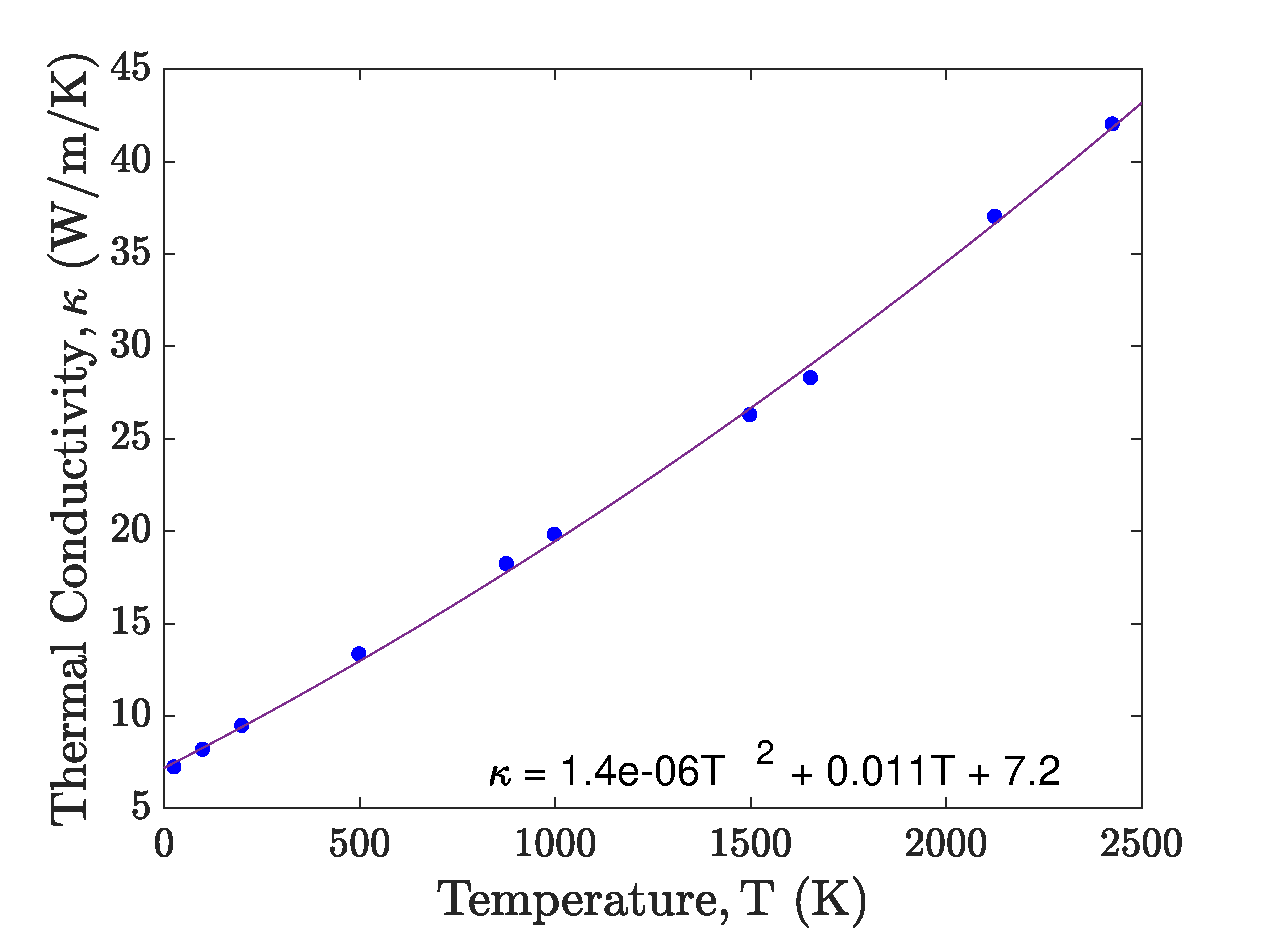
\includegraphics[width=0.42\textwidth]{./Figures/kappa_fit}
\end{center}
\caption{A second degree polynomial fit to specific heat~($C_p$), and thermal conductivity~($\kappa$) data
for a temperature range, [20,1655](K). Note that the data provided in~\cite{Fu:2014} was used to determine
the coefficients of the regression fit.}
\label{fig:Cp_kappa}
\end{figure}
%
Hence, a total of 12 parameters~($\bm{\theta}$) are mapped to the stress field including coefficients of the polynomial fits
corresponding to $C_p$ and $\kappa$. A uniform prior: $[0.9\bm{\theta}^\ast, 1.1\bm{\theta}^\ast]$, 
where $\bm{\theta}^\ast$ denotes a vector of nominal values,
is considered for each parameter. Nominal values of the mechanical properties: $Y$, $E$, and $\rho$ are provided
in Table~\ref{tab:matProp}. Nominal values of the process control parameters and temperature coefficients for
the thermal properties are provided in Table~\ref{tab:remain}.
%
\begin{table}[htbp]
\centering
\caption{EBM process control parameters and temperature coefficients for $C_p$~($C_i$'s) and $\kappa$~($D_i$'s).}
\label{tab:remain}
\vspace{1mm}
\begin{tabular}{ ll }
\toprule
Scan Speed, $v$~(mm/s) & 500 \\
Beam Power, $P$~(W) & 160 \\
Pre-heat Temperature, $T_0$~(C) & 650 \\
Specific heat, $C_p$ = $C_0+C_1T+C_2T^2$~(J/kg/K) & 540~($C_0$),0.43~($C_1$),$-3.2\times 10^{-5}$~($C_2$) \\
Thermal Conductivity, $\kappa$ = $D_0+D_1T+D_2T^2$~(W/m/K) & 7.2~($D_0$),0.011~($D_1$),$1.4\times 10^{-6}$~($D_2$) \\
\bottomrule
\end{tabular}
\end{table}
%%%

Residual stress is initially computed at the x$^c$-z$^c$ plane for 10 pseudorandom samples in the 12-dimensional
input domain. Stress data is simulated on a 2-dimensional non-uniform grid comprising 32 points along the
length~(x$^c$) and 14 points along the height~(z$^c$) as highlighted in Figure~\ref{fig:RS_comp}~(left).
As mentioned earlier in Section~\ref{sec:model}, a 
finer mesh is used near the part surface since sharp thermal gradients lead to a larger amount of stress
in this region as shown in Figures~\ref{fig:subSmises} and~\ref{fig:RS_comp}.  Following the flow diagram
in Figure~\ref{fig:fd}, the first step involves a principal component analysis on the field data. 
Algorithm~\ref{alg:pca}) is used for this purpose. However, the reconstructed field failed
the verification and the validation tests in this case, i.e. $\varepsilon_0^{\text{ver}}$ and $\varepsilon_0^{\text{val}}$
were greater than 0.1. A new set of 5 model realizations were added at subsequent iterations and the iterative
procedure was observed to converge in 2 iterations. Error estimates for each iteration are provided in
Table~\ref{tab:error}.
%
\begin{table}[htbp]
\centering
\caption{Convergence of the surrogate model as a function of iterations and sample size.}
\label{tab:error}
\vspace{1mm}
\begin{tabular}{ ccll}
\toprule
Iteration &  Sample Size & $\varepsilon_i^{\text{ver}}$ & $\varepsilon_i^{\text{val}}$\\
0 & 10 & 0.06 & 0.31 \\
1 & 15 & 0.09 & 0.28 \\
2 & 20 & 0.04 & 0.07\\
\bottomrule
\end{tabular}
\end{table}


In Figure~\ref{fig:pca}, we plot the reconstruction error, $\varepsilon_\mathcal{R}^\infty$ against the number of
principal components, $K$. 
%
\begin{figure}[htbp]
\begin{center}
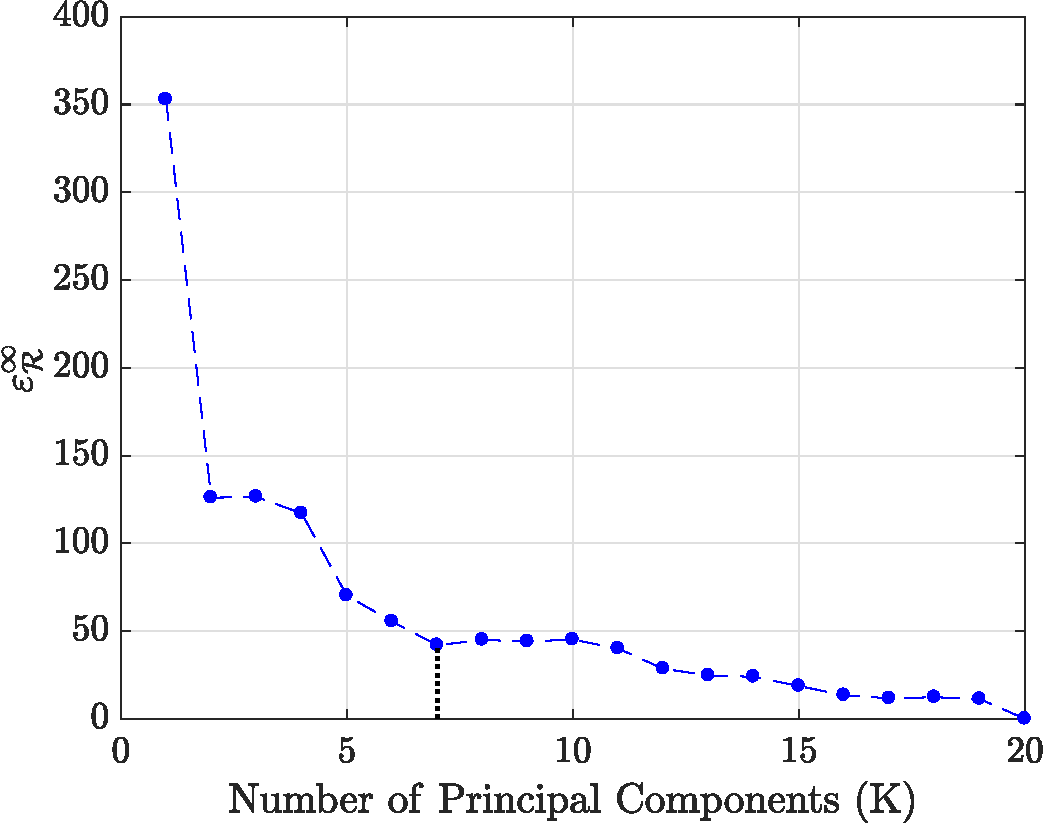
\includegraphics[width=0.42\textwidth]{./Figures/error_PCA}
\end{center}
\caption{A plot of the reconstruction error, $\varepsilon_\mathcal{R}^\infty$ as a function of the
number of principal components obtained using the iterative PCA approach in Algorithm~\ref{alg:pca}.}
\label{fig:pca}
\end{figure}
%
As expected, $\varepsilon_\mathcal{R}^\infty$ is observed to mostly decrease with the number of components. 
A monotonic behavior is not expected since the components only capture partial information in the data. It 
appears that most of the information is captured using 20 components since the error is almost 0. However,
building the surrogate for 20 features would potentially entail a large computational effort depending upon the
application. Here, we consider that $K^\ast$ = 7 components are optimal since the error plateaus as the number of
components increase from 7 to 10 indicating diminishing returns. Thus, the residual stress field is reconstructed
using a surrogate for each of these $K^\ast$ components~($\mathcal{Z}_i$'s, $i = 1,2,\ldots,K^\ast$).
The dimensionality of the output space is therefore reduced 
from $\mathbb{R}^{14\times 32=448}\rightarrow \mathbb{R}^7$. We now shift our focus on dimension reduction
in the input space.

As discussed earlier in~\ref{sub:as}, each feature can be expressed as a function of $\bm{\theta}$ in the physical
space. Note that $\bm{\theta}:\{\bm{\theta_P}\cup\bm{\theta_M}\cup\bm{\theta_T}\}$. An active subspace computation
was performed using a regression-based approach~\cite{Constantine:2015, Vohra:2019}
for estimating the gradient and the available set of 20 realizations for each $\mathcal{Z}_i$. 
The eigenvalue spectrum of the matrix, $\hat{\mathbb{C}_i}$ for each $\mathcal{Z}_i$ is shown in Figures~\ref{fig:as1}
and~\ref{fig:as2}.
The variability of a given $\mathcal{Z}_i$ in terms of the active variables, $\bm{\eta}$ regarded as the sufficient summary
plot~(SSP) is also included in each case.
%
\begin{figure}[htbp]
\begin{center}
%\begin{subfigure}{0.5\textwidth}
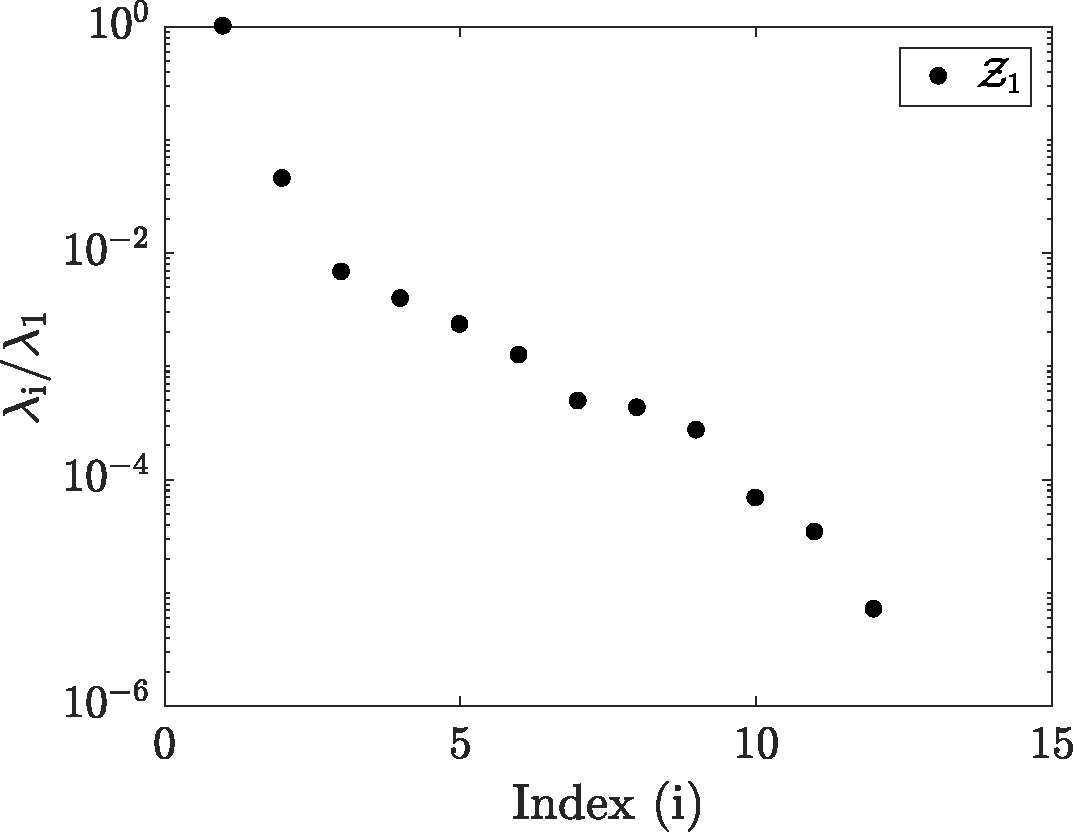
\includegraphics[width=0.35\textwidth]{./Figures/eig_Zf1} 
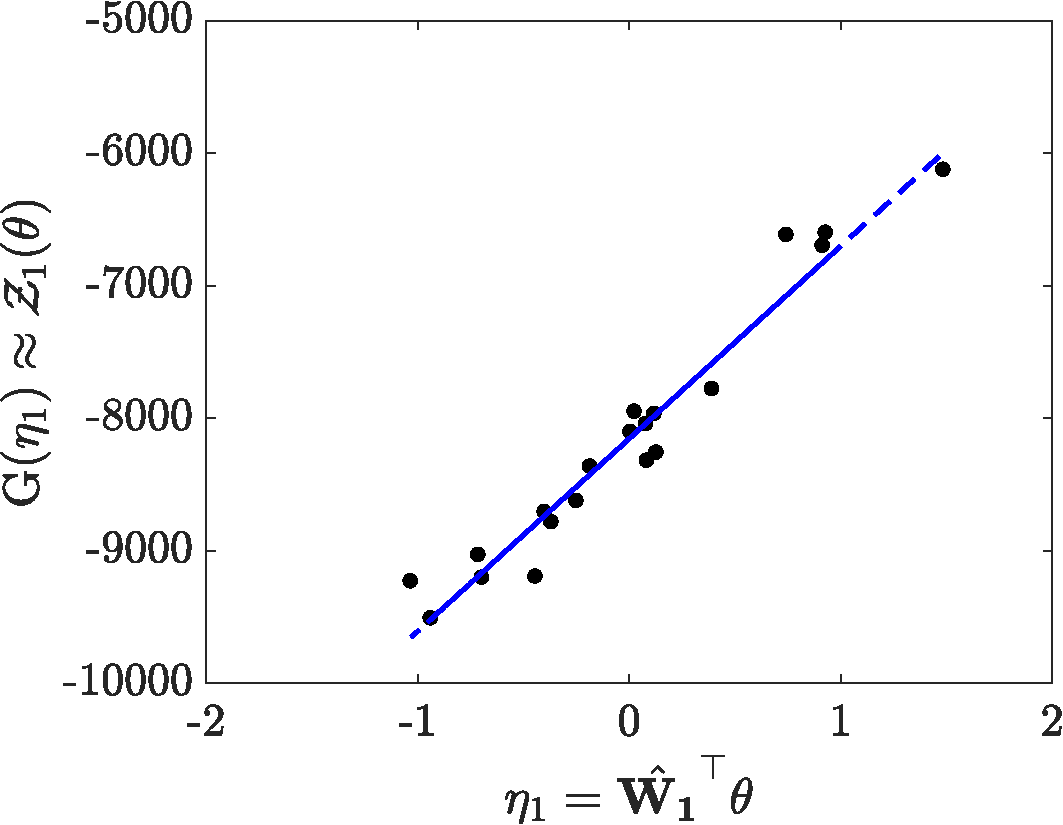
\includegraphics[width=0.35\textwidth]{./Figures/SSP_Zf1} 
\\
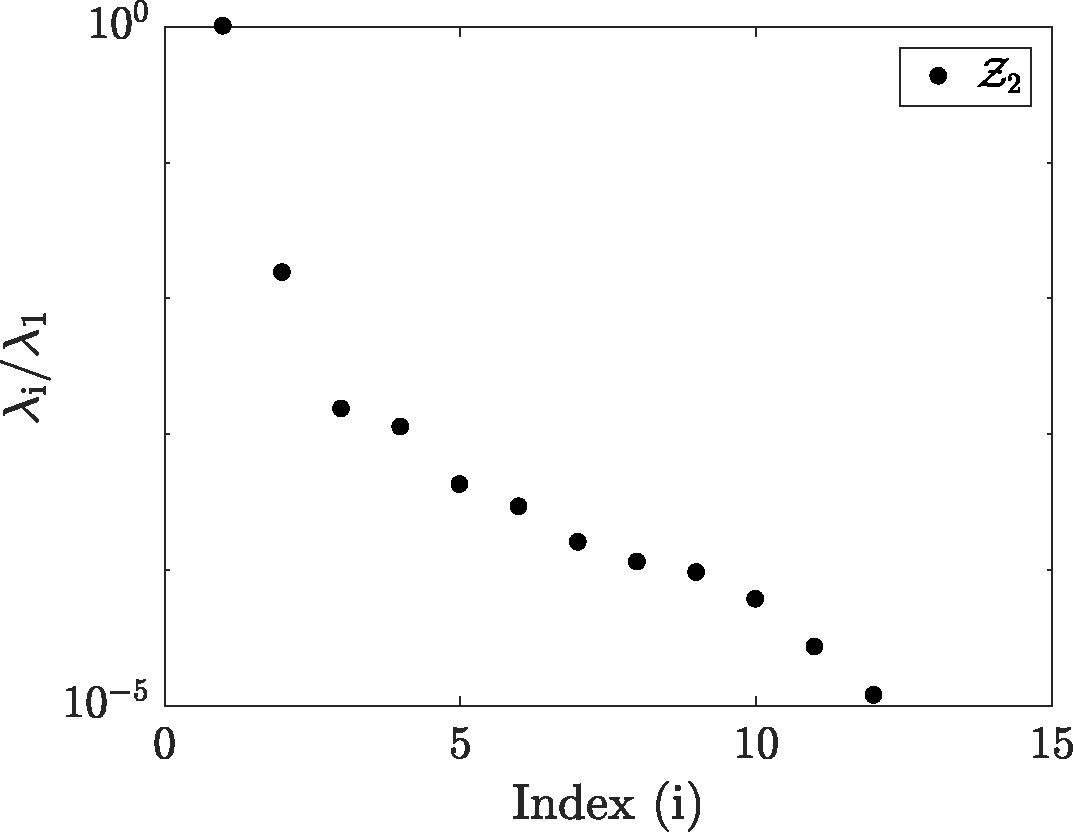
\includegraphics[width=0.35\textwidth]{./Figures/eig_Zf2} 
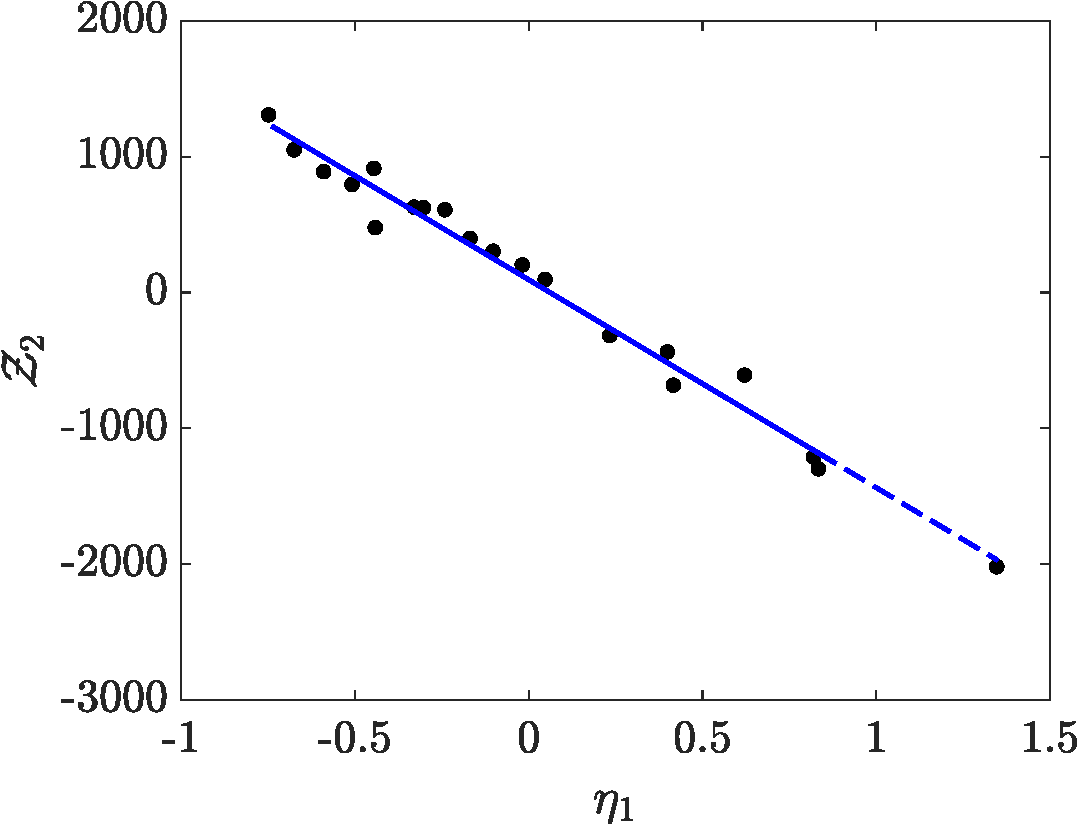
\includegraphics[width=0.35\textwidth]{./Figures/SSP_Zf2} 
\\
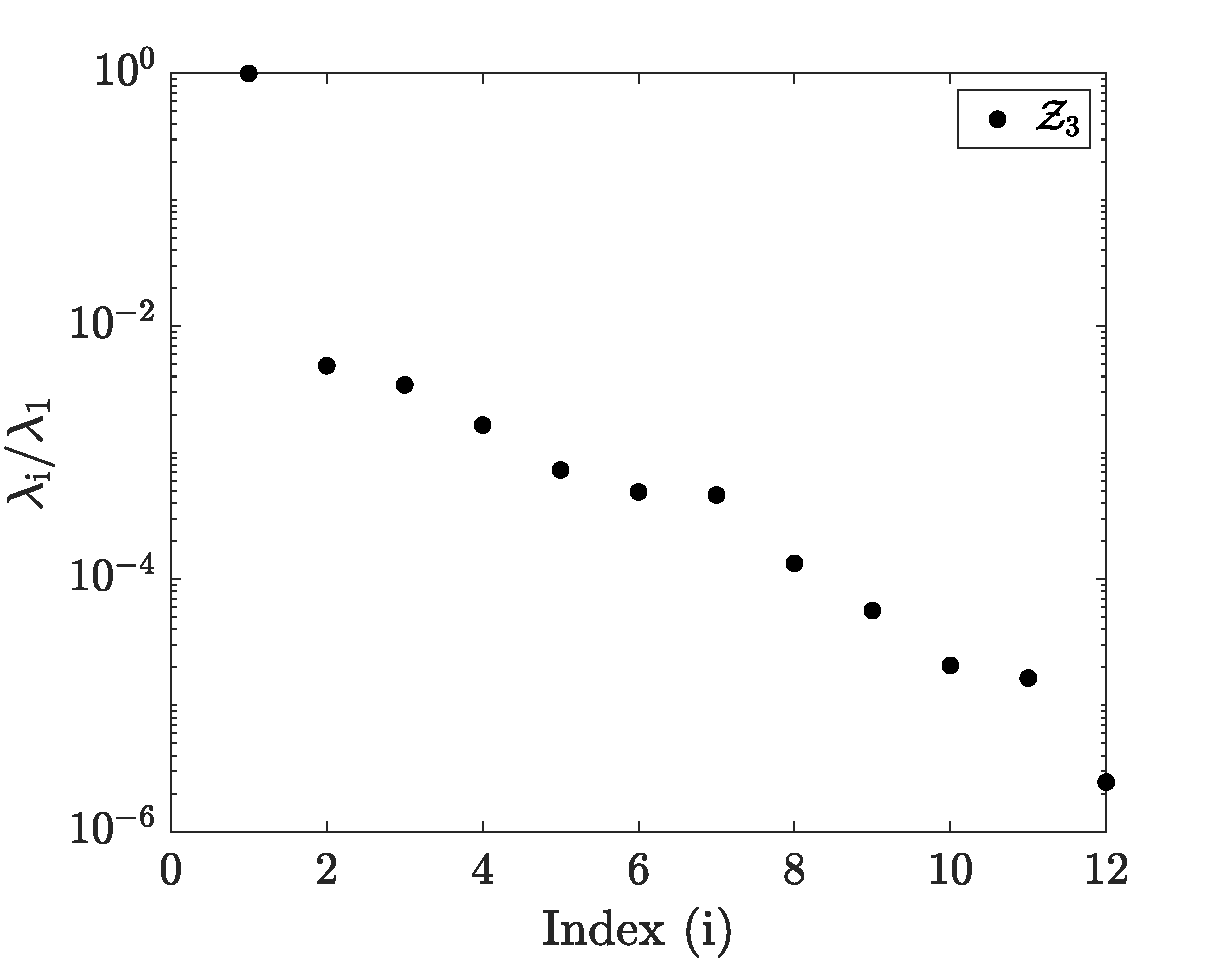
\includegraphics[width=0.35\textwidth]{./Figures/eig_Zf3} 
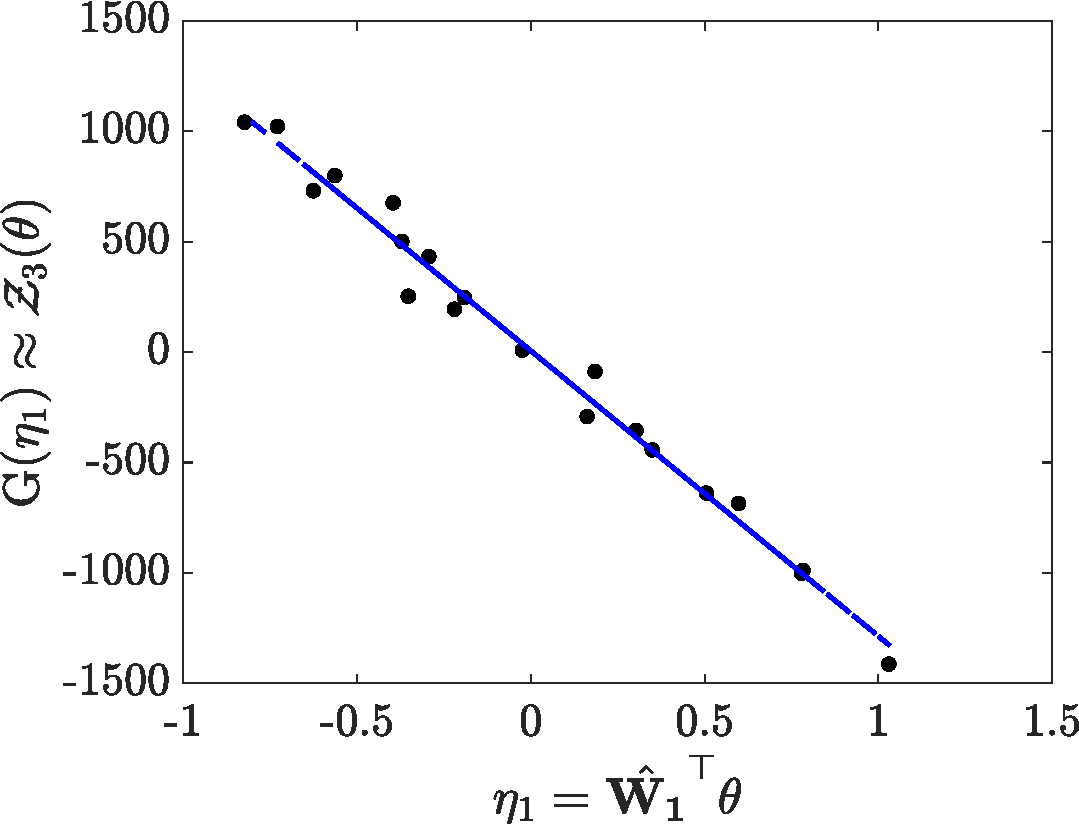
\includegraphics[width=0.35\textwidth]{./Figures/SSP_Zf3} 
\\
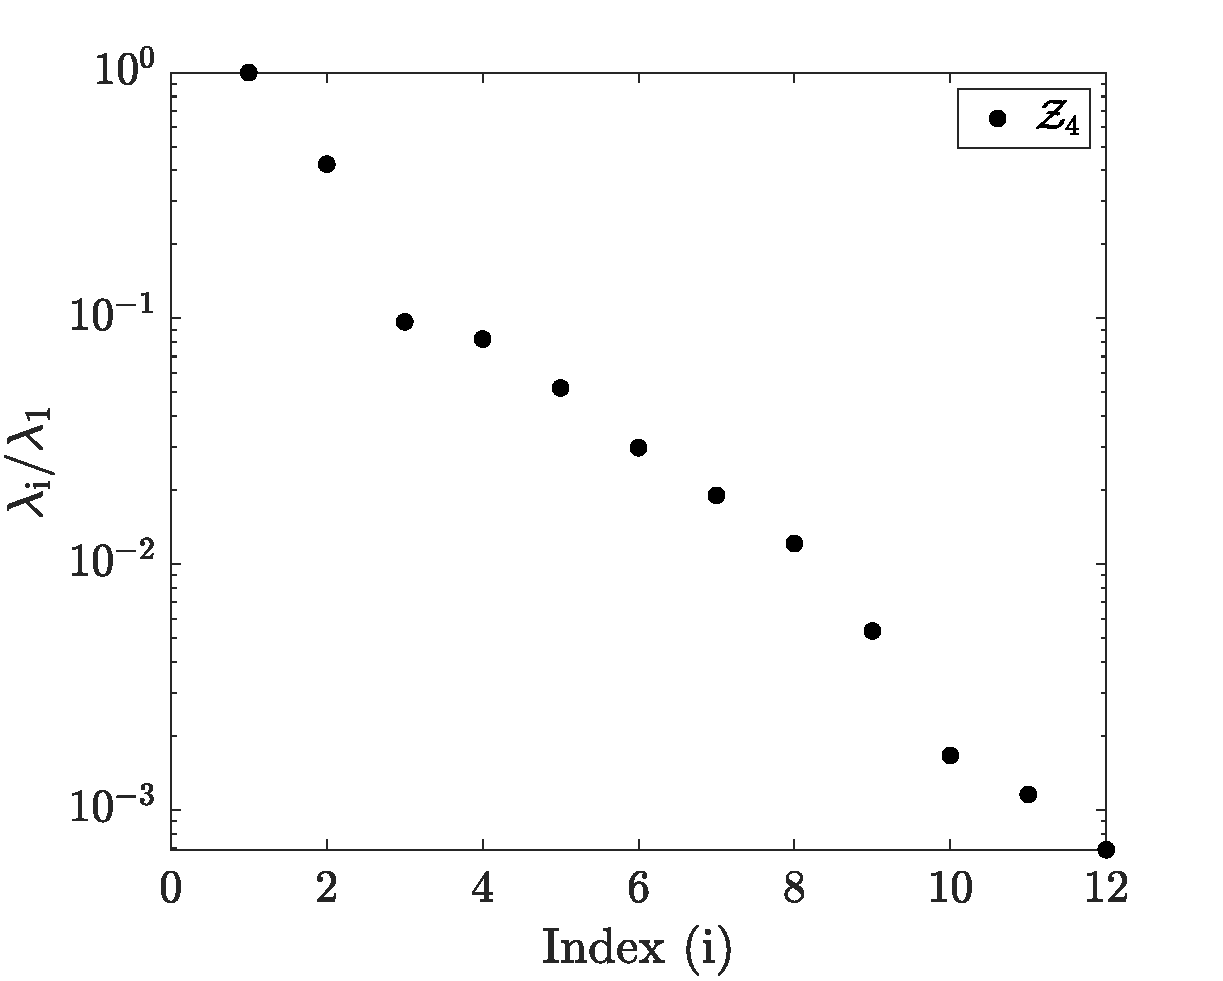
\includegraphics[width=0.35\textwidth]{./Figures/eig_Zf4} 
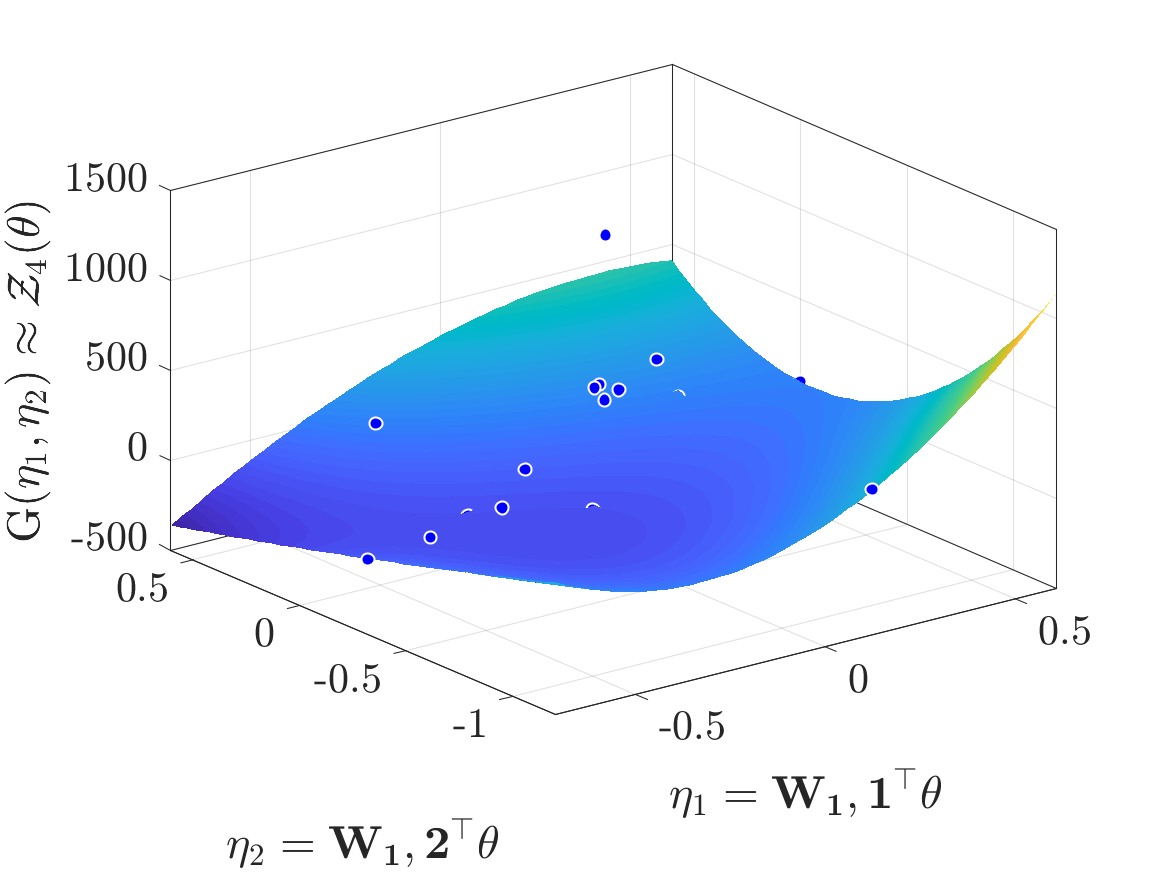
\includegraphics[width=0.35\textwidth]{./Figures/SSP2D_Zf4} 
\end{center}
\caption{Eigenvalue spectrum~(left) and the corresponding SSP~(right) for $\mathcal{Z}_i, i=1,2,3,4$.
A straight line fit in the case of $\mathcal{Z}_{1,2,3}$ and a
2D polynomial surface fit in the case of $\mathcal{Z}_4$ is used as a surrogate model as illustrated.}
\label{fig:as1}
\end{figure}
%
%
\begin{figure}[htbp]
\begin{center}
%\begin{subfigure}{0.5\textwidth}
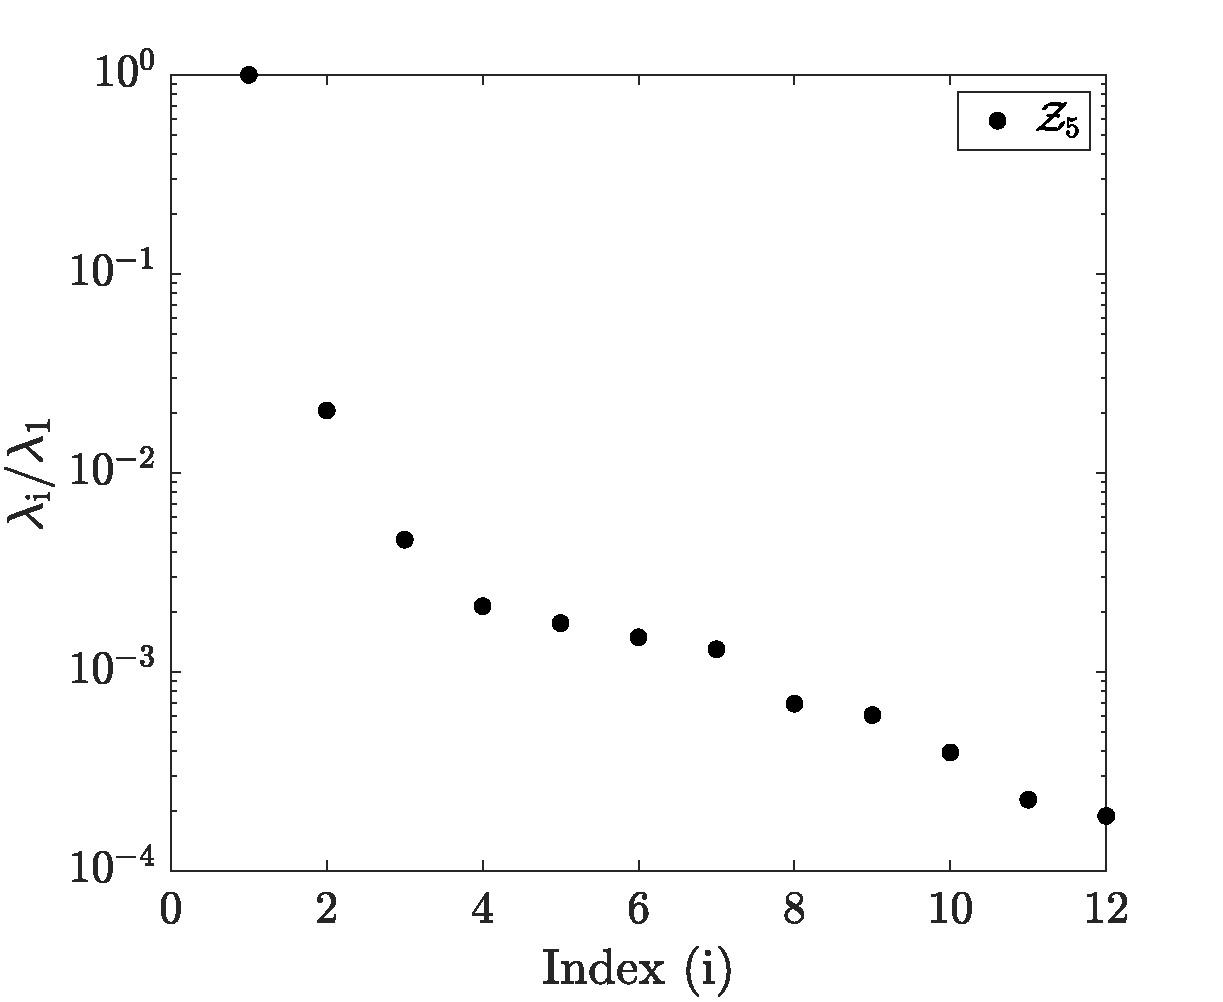
\includegraphics[width=0.35\textwidth]{./Figures/eig_Zf5} 
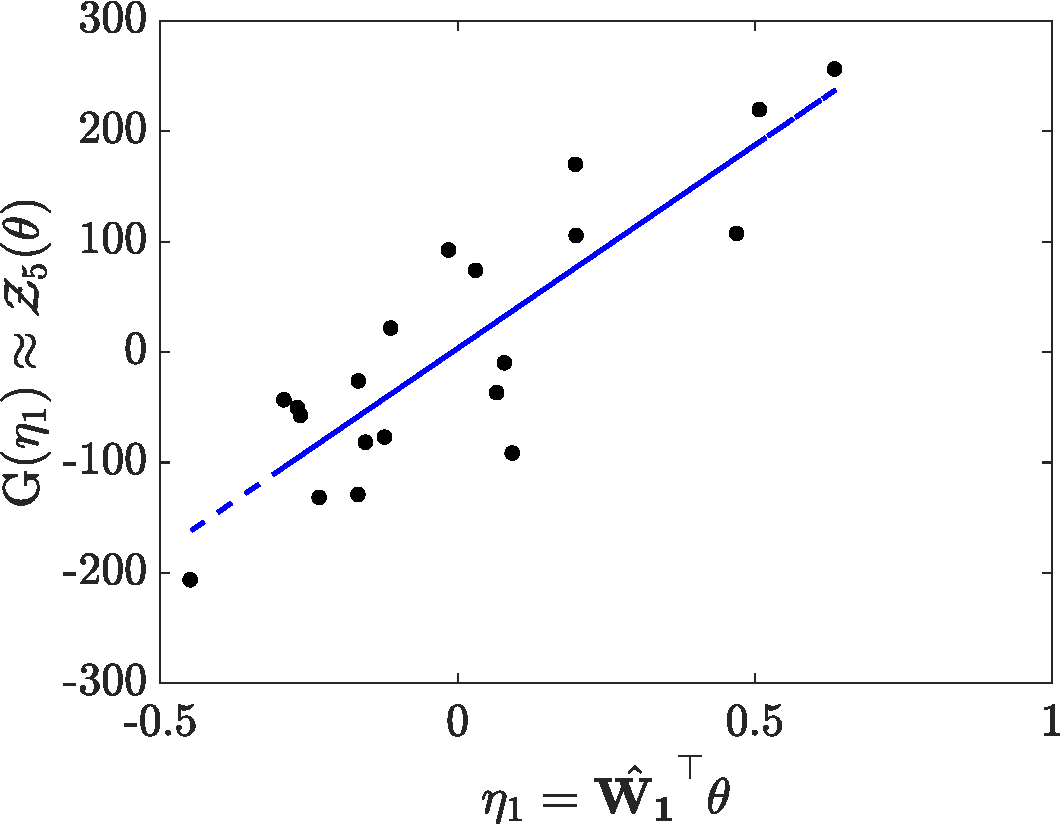
\includegraphics[width=0.35\textwidth]{./Figures/SSP_Zf5} 
\\
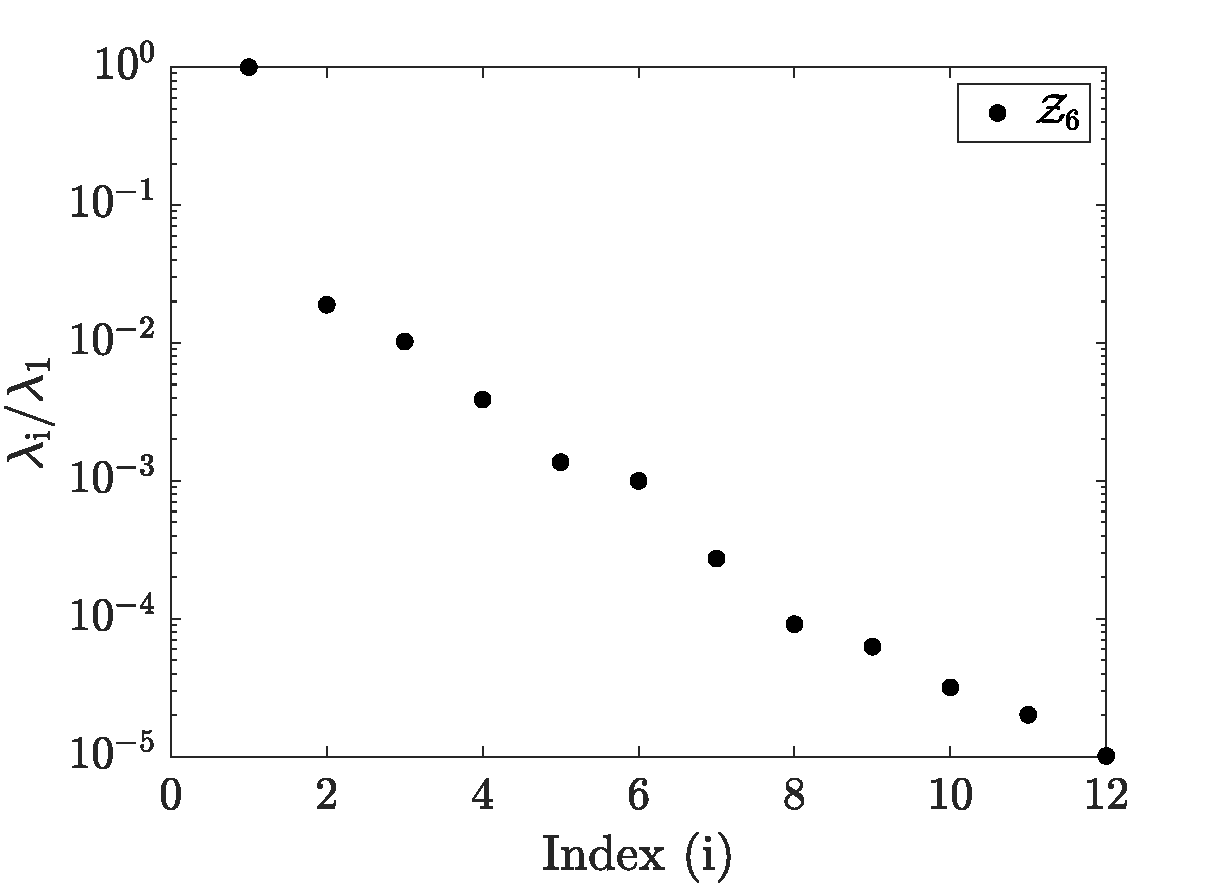
\includegraphics[width=0.35\textwidth]{./Figures/eig_Zf6} 
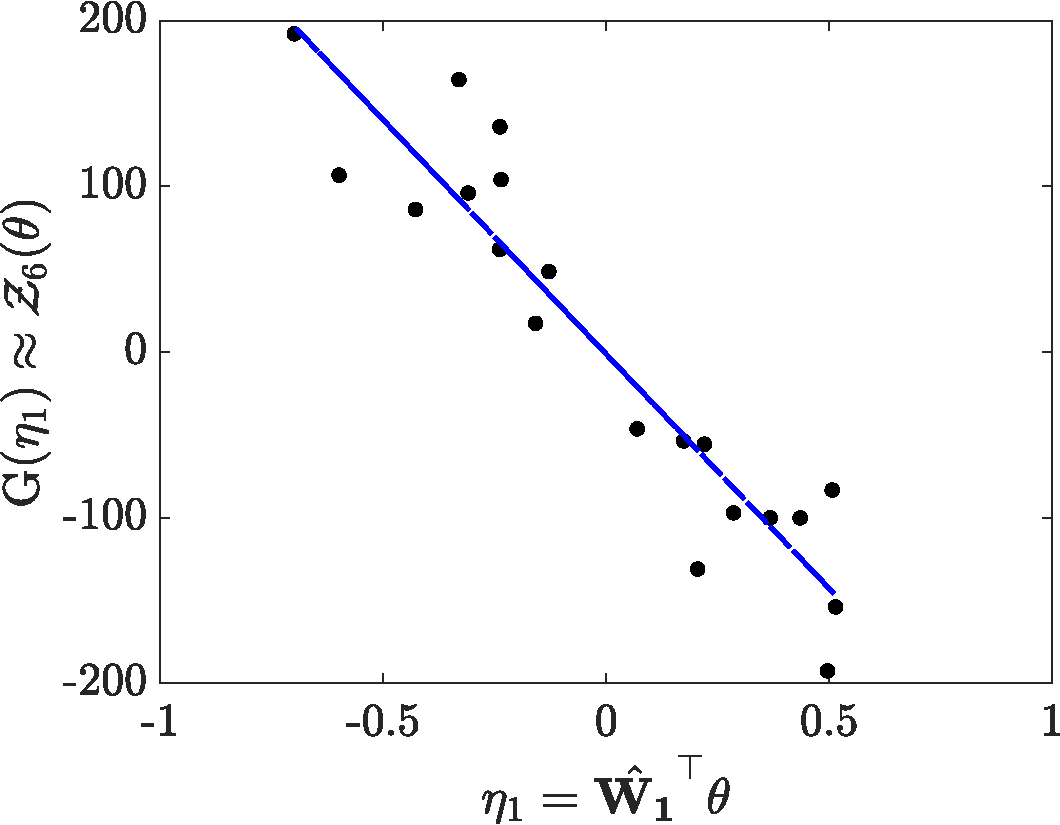
\includegraphics[width=0.35\textwidth]{./Figures/SSP_Zf6} 
\\
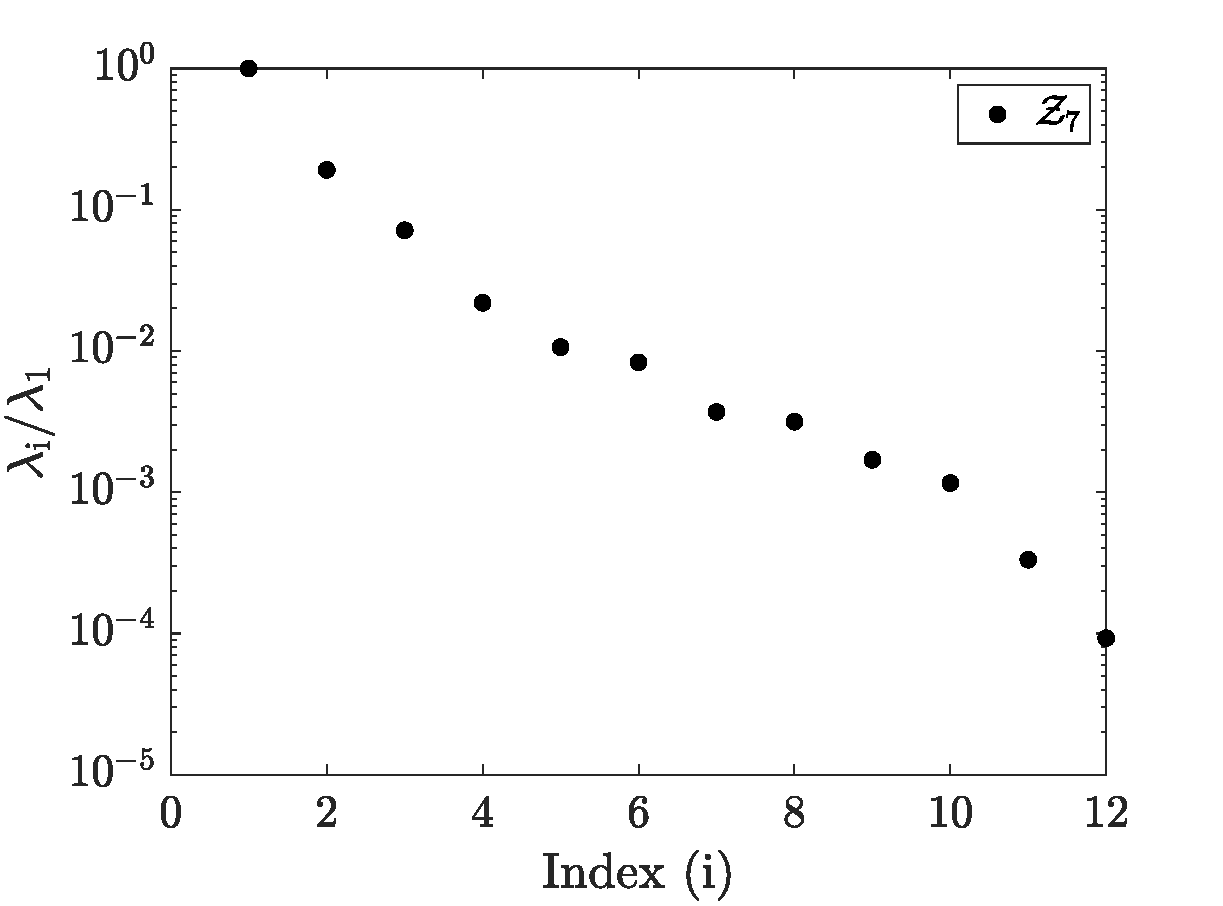
\includegraphics[width=0.35\textwidth]{./Figures/eig_Zf7} 
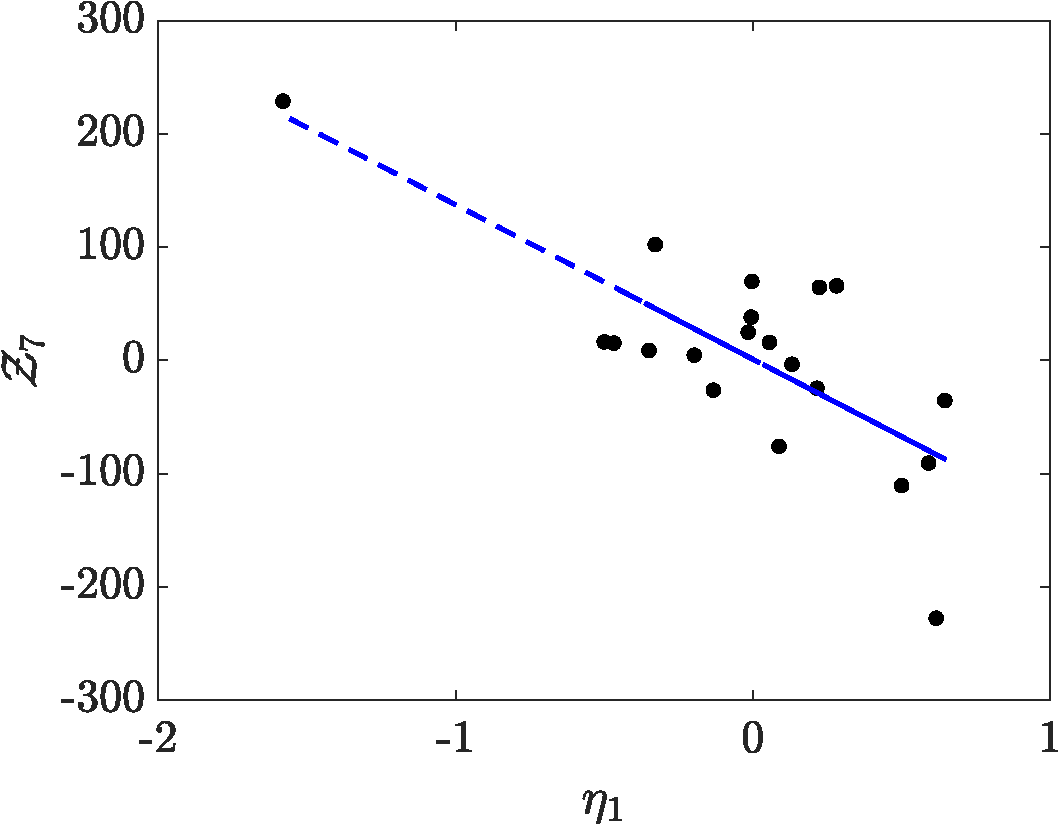
\includegraphics[width=0.35\textwidth]{./Figures/SSP_Zf7} 
\end{center}
\caption{Eigenvalue spectrum~(left) and the corresponding SSP~(right) for $\mathcal{Z}_i, i=5,6,7$.
A straight line fit to the SSP is used as a surrogate model as illustrated in each case.}
\label{fig:as2}
\end{figure}
%
From these plots, it is observed that in all cases except $\mathcal{Z}_4$, a 1-dimensional active
subspace captures the variability in the feature with reasonable accuracy. More specifically, the
eigenvalue spectrum exhibits a significant jump between the first and second eigenvalue. Consistent
with these observations, a straight-line fit to the realizations of the feature in the SSP is observed to be
reasonably accurate. In the case of $\mathcal{Z}_4$, $\lambda_1$ and $\lambda_2$ are comparable, and
a significant jump exists between $\lambda_2$ and $\lambda_3$. Therefore, a 2-dimensional active
subspace is considered in this case as shown. Polynomials of degrees 3 and 2 along $\eta_1$ and
$\eta_2$ respectively were used to construct the regression surface. The regression-fits in each case
serves as a surrogate for the corresponding feature, $\mathcal{Z}_i$. Therefore, a sample $\bm{\xi}_i$
corresponding to $\bm{\theta}_i$ in the physical space is propagated through each surrogate to estimate
$\mathcal{Z}_i$'s and hence, the residual stress field as shown using a flow diagram in Figure~\ref{fig:re}.
The individual surrogates for $\mathcal{Z}_i$'s thus constitute the overall surrogate model that maps the 
physical variables to the stress field. We will refer to this overall surrogate model as the \textit{composite
surrogate} in the remainder of this paper. 

Dimension reduction in the input space is therefore found to be from $\mathbb{R}^7\rightarrow\mathbb{R}^2$.
Therefore, using the proposed PCAS method, significant dimension reduction in both input and output
spaces is accomplished leading enormous gains in computational efficiency for the considered application.

\subsubsection{Surrogate Verification and Validation}
\label{subsub:vnv}

As mentioned earlier in this section, 20 model realizations were needed to obtain a surrogate model with
reasonable accuracy with respect to the reconstructed residual stress field in the x$^c$-z$^c$ plane. 
Specifically, the verification and validation errors were found to be approximately 0.04 and 
0.07 respectively. In other words, the stress field reconstructed using the
composite surrogate model achieves an accuracy of about 7$\%$ on average. Although these error estimates
are based on a relatively small sample size, they seem reasonable considering that the validation test samples
were generated using Latin hypercube sampling (LHS) that explores the entire input domain more uniformly
as compared to Monte Carlo sampling. Therefore, the PCAS approach appears to provide a reasonably 
accurate surrogate coupled with enormous computational gains which makes the analyses pertaining to
the present application affordable. 

Figure~\ref{fig:RS_comp} illustrates a side-by-side comparison of stress distribution in the $x^c$-z$^c$ plane,
computed using the FEM~(left) with those generated using the composite surrogate~(right) using the same
set of input conditions. The two plots
are observed to be in close agreement with each other.  
%
\begin{figure}[htbp]
\begin{center}
\begin{subfigure}{0.15\textwidth}
\vspace{10mm}
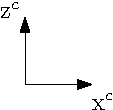
\includegraphics[width=0.5\textwidth]{./Figures/xczc} 
\end{subfigure}
\hspace{-1.5cm}
\begin{subfigure}{0.35\textwidth}
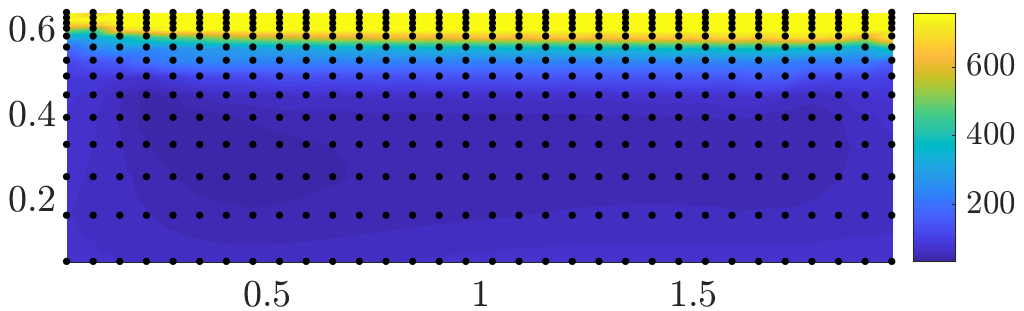
\includegraphics[width=1.0\textwidth]{./Figures/origZ_sam13} 
\end{subfigure}
\hspace{0.25cm}
\begin{subfigure}{0.35\textwidth}
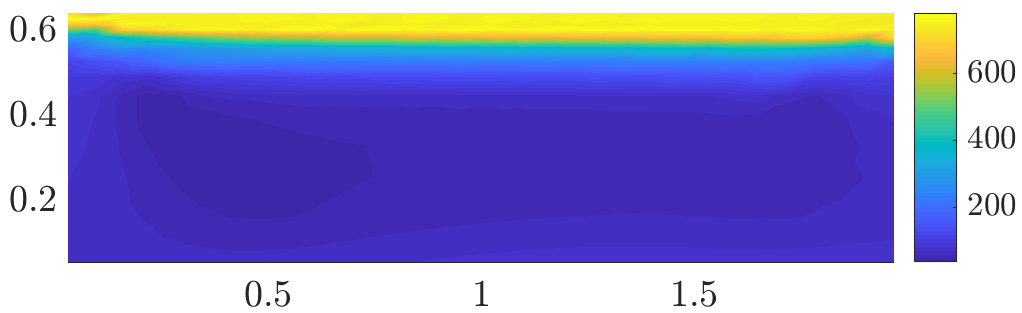
\includegraphics[width=1.0\textwidth]{./Figures/recZ_sam13} 
\end{subfigure}
\end{center}
\caption{Left: Residual stress field in the $x^c$-z$^c$ plane as generated using the Abaqus model with inputs, 
$\bm{\theta}_p$. The grid points in the 2D mesh used for finite element simulations are also highlighted. 
Right: Reconstructed stress field using the surrogate model using the same set of parameters. }

%: $v=535.23$~mm/s, $P$=148.27~W,
%$T_0$=641.03~K, $Y$=777.74~MPa, $E$=99.16~GPa, $\rho$=4187.25~kg/m$^3$, $C_0$=546.43, $C_1$=0.47,
%$C_2$~=~-~3.07$\times$10$^{-5}$, $D_0$=6.84, $D_1$=0.01, $D_2$=1.47$\times$10$^{-6}$.}
\label{fig:RS_comp}
\end{figure}

\subsubsection{Hotspot Identification}
\label{subsub:hotspot}

As mentioned earlier in Section~\ref{sec:intro}, a large amount of residual stress severely impacts part
performance due to sub-optimal mechanical properties, reduced fatigue life, and geometrical inaccuracy. 
Identification of `stress hotspots' could thus be conceived as an important step in the manufacturing process.
Owing to the transient nature of the process conditions, material microstructure, and part configuration,
it would not be practicable to use the FEM. The surrogate model constructed using the PCAS method
proposed in this work could instead be used for the purpose.

For the present analysis, we focus on the hotspots in the $x^c$-z$^c$ plane, and any point in the 2D mesh
where the residual stress exceeds a threshold is considered as the hotspot. Figure~\ref{fig:hs} illustrates the 
location of the hotspots and associated stress values in the $x^c$-z$^c$ plane, for a particular set of
input conditions. A threshold value of 640~MPa is used. 
%
\begin{figure}[htbp]
\begin{center}
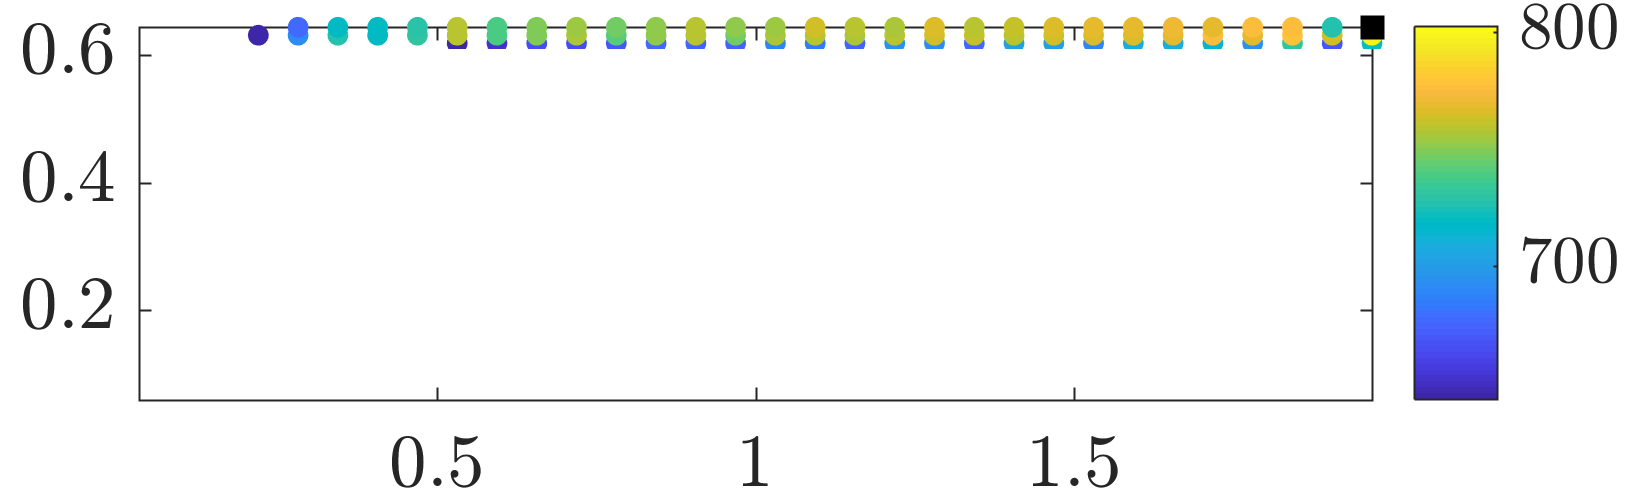
\includegraphics[width=0.42\textwidth]{./Figures/loc_hotspot10}
\end{center}
\caption{Location of the hotspots in the AM part and corresponding estimates of the von Mises stress
are indicated by means of a colorbar. The location of the peak stress is also shown using a black square.}
\label{fig:hs}
\end{figure}
%
As expected, the hotspots are located near the top surface of the part that experiences sharp temperature
gradients. For the purpose of identifying a global hotspot, the residual stress
field in the $x^c$-z$^c$ plane is simulated for 10$^6$ pseudorandom samples, generating using LHS
in the 12-dimensional input domain. Thus, stress distribution is obtained at each point in the mesh. 
The specific grid point with the maximum mean stress is regarded as the \textit{global hotspot},
denoted as P. Our findings reveal that P is in fact located at the top right corner of the $x^c$-z$^c$
plane, consistent with the location of the square in Figure~\ref{fig:hs}.
Figure~\ref{fig:kde_S} shows the PDF of stress distribution at point P. 
%
\begin{figure}[htbp]
\begin{center}
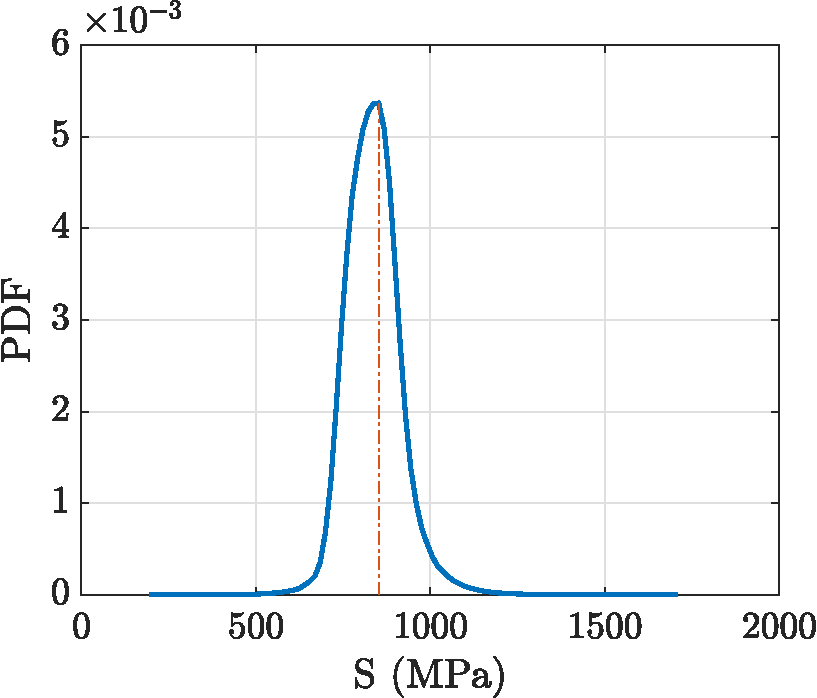
\includegraphics[width=0.42\textwidth]{./Figures/kde_S_mumax}
\end{center}
\caption{Probability density function~(PDF) of von Mises stress at P, generated using kernel density estimation in 
Matlab. The distribution is based on 10$^6$ evaluations and the mode value is estimated as 852.31~MPa.}
\label{fig:kde_S}
\end{figure}

\subsection{Global Sensitivity Analysis}
\label{sub:gsa}

The composite surrogate is further used for the purpose of global sensitivity analysis~(GSA). %
GSA is performed with respect to the stress value at point $P$, identified as the global hotspot
for residual stress in the $x^c$-z$^c$ plane as discussed earlier in~\ref{subsub:hotspot}. 

As mentioned earlier, the set of inputs in the physical space, $\bm{\theta}$ is classified into three
categories: process control parameters~($\bm{\theta_P}$), mechanical properties~($\bm{\theta_M}$), and
thermal properties~($\bm{\theta_T}$) of the alloy~(Ti6Al4V) used to manufacture the AM part. We focused
our efforts on determining the relative importance of $\bm{\theta_P}$, $\bm{\theta_M}$, and $\bm{\theta_T}$
wherein the individual parameters in each category are grouped together. Additionally, we investigate
relative importance of the process
control parameters and the material properties, i.e. $\bm{\theta_M}$ and $\bm{\theta_T}$ grouped together.
Such analyses with grouped variables would help focus the manufacturer's attention on the key
contributors to the variability in residual stress. For instance, depending upon the sensitivity estimates, the
manufacturer could focus on optimizing either the mechanical properties, thermal properties, or
the process control variables for minimizing the uncertainty in residual stress prediction. 
More importantly, optimizing the key contributors to the variability in residual stress would help maximize the reliability
of the finished product. 
 GSA was performed by estimating the main-effect and the total-effect Sobol' sensitivity
indices at 10$^5$ samples in the input domain using an algorithm based on 
Monte Carlo sampling~(MCS)~\cite{Sobol:2001}. The composite
surrogate was used to make the computations tractable. The estimated sensitivities for the two cases
are plotted in Figure~\ref{fig:gsa}.
%
\begin{figure}[htbp]
\begin{center}
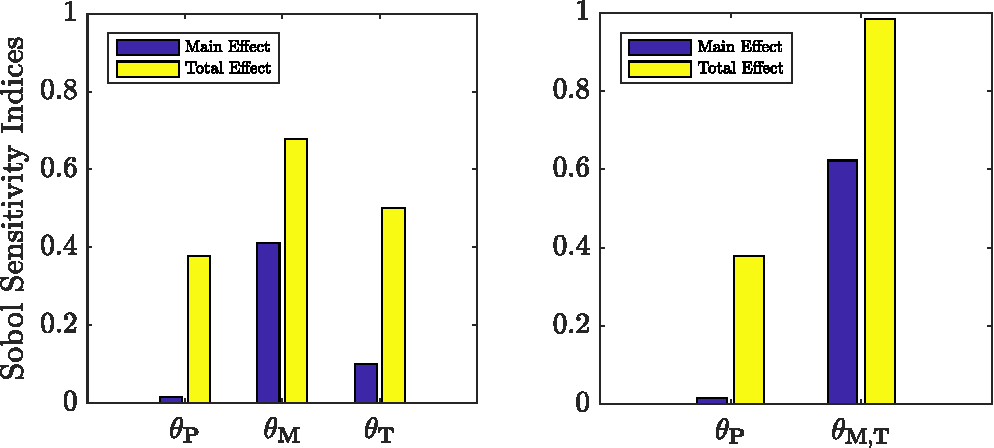
\includegraphics[width=0.65\textwidth]{./Figures/grouped_GSA}
\end{center}
\caption{Left: Sobol' sensitivity indices for the set of inputs grouped as process variables~($\bm{\theta_P}:v,P,T_0$), 
mechanical properties~($\bm{\theta_M}:Y,E,\rho$), and thermal properties~($\bm{\theta_T}:C_p,\kappa$).
Right: Sobol' sensitivity indices for the set of inputs grouped as process variables~($\bm{\theta_P}$), and material 
properties~($\bm{\theta_{M,T}}$).}
\label{fig:gsa}
\end{figure}
%
Several inferences can be made: The residual stress at P is most sensitive to the mechanical properties, followed 
by thermal properties of the alloy. Sensitivity towards the process control parameters is found to be relatively small. 
However, it must be noted that the interactions between $\bm{\theta_P}$, $\bm{\theta_M}$, and $\bm{\theta_T}$
are significantly large. Hence, the total-effect index of $\bm{\theta_P}$ indicates that the sensitivity towards the 
process variables is substantial. Therefore, optimizing the process parameters for minimizing residual
stress in the AM part could help improve its performance characteristics. 
Note that these results are dependent on the choice of nominal values as well as considered intervals
for the uncertain inputs. 

\subsection{Reliability Prediction}
\label{sub:reliability}

Reliability prediction involves estimating the probability of failure~($p_f$) of the AM part
corresponding to a defined failure criterion. Here, we estimate~$p_f$ based on the residual 
stress estimate at any location in
the part exceeding a given threshold. In other words, we aim to ensure that the residual stress
in the part does not exceed an upper bound and therefore, the performance characteristics of
the AM part are not severely degraded. Once again, we exploit the composite surrogate to
numerically estimate~$p_f$ as follows:
%
\be
\hat{p}_f = \frac{1}{N}\sum\limits_{k=1}^{N} \mathbb{H}\left[S^\ast-\max(\hat{\mat{S}})\right],
\ee
\label{eq:pf}
%
where $\hat{p}_f$ is the approximation to $p_f$, $N$ denotes the number of samples, $S^\ast$
denotes the limiting stress value, and $\max(\hat{\mat{S}})$ denotes the peak stress in the
x$^c$-z$^c$ plane based on the surrogate prediction. $\mathbb{H}[]$
is a Heaviside unit step function that assumes a value 1 for a positive argument and 0 for
a negative argument.
To ensure that $\hat{p}_f$ is a resonable approximation, it is estimated
using 10$^6$ samples in the input domain. Based on surrogate predictions at the generated set of samples,
the probability of failure using $S^\ast$~=~900~MPa is estimated to be 0.177. 


















































 
